\documentclass{../../text-style}

\texttitle{Лекция 11: Рефакторинг}

\begin{document}

\maketitle
\thispagestyle{empty}

\attribution{Тимофей Александрович Брыксин, бывш. доцент кафедры системного программирования СПбГУ}

Рефакторинг представляет собой процесс такого изменения программной системы, при котором не меняется внешнее поведение кода, но улучшается его внутренняя структура. Это способ систематического приведения кода в порядок, при котором шансы появления новых ошибок минимальны. В сущности, при проведении рефакторинга кода вы улучшаете архитектуру и код уже после того, как они написаны.

<<Улучшение кода после его написания>>~--- непривычная для многих фигура речи. В классическом понимании разработки программного обеспечения мы сначала создаем дизайн системы, а потом пишем код. Сначала создается хороший дизайн, а затем происходит кодирование. Но со временем код модифицируется, и целостность системы, соответствие ее структуры изначально созданному дизайну постепенно ухудшаются.

Рефакторинг представляет собой противоположную практику. С ее помощью можно взять плохой проект и переделать его в хорошо спроектированный код. Каждый шаг этого процесса довольно прост: перемещается поле из одного класса в другой, изымается часть кода из метода и помещается в отдельный метод, какой-то код перемещается в иерархии в том или другом направлении. Однако суммарный эффект таких небольших изменений может радикально улучшить проект. Это прямо противоположно обычному явлению постепенного распада программы.

При проведении рефакторинга оказывается, что соотношение разных этапов работ изменяется. Проектирование непрерывно осуществляется во время разработки, а не выполняется целиком заранее. При реализации системы становится ясно, как можно улучшить ее проект. Происходящее взаимодействие приводит к созданию программы, качество проекта которой остается высоким по мере продолжения разработки.

Следует более подробно остановиться на некоторых местах в данных определениях. Во-первых, цель рефакторинга~--- упростить понимание и модификацию программного обеспечения. Можно выполнить много изменений в программном обеспечении, в результате которых его видимое поведение изменится незначительно или вообще не изменится. Рефакторингом будут только такие изменения, которые сделаны с целью облегчения понимания исходного кода. Противоположным примером может служить оптимизация производительности. Как и рефакторинг, оптимизация производительности обычно не изменяет поведения компонента (за исключением скорости его работы), она лишь изменяет его внутреннее устройство. Цели, однако, различны. Оптимизация производительности часто затрудняет понимание кода, но она необходима для достижения желаемого результата.

Второе обстоятельство, которое хочется отметить, заключается в том, что рефакторинг не меняет видимого поведения программного обеспечения. Оно продолжает выполнять прежние функции. Никто, ни конечный пользователь, ни программист, не сможет сказать по внешнему виду, что что-то изменилось. В процессе разработки программного обеспечения может оказаться необходимым часто переключаться между двумя видами работы. Попытавшись добавить новую функцию, можно обнаружить, что это гораздо проще сделать, если изменить структуру кода. Тогда следует на некоторое время переключиться на рефакторинг. Улучшив структуру кода, можно добавлять новую функцию. А добившись ее работы, можно заметить, что она написана способом, затрудняющим ее понимание, тогда вы снова переключаетесь и занимаетесь рефакторингом. Все это может происходить в течение десяти минут, но в каждый момент вы должны понимать, которым из видов работы заняты. Чтобы не допускать лишних ошибок, важно эти виды деятельности не смешивать.

\section{Зачем нужно проводить рефакторинг?}

Рефакторинг не является <<серебряной пулей>> или лекарством от всех болезней. Тем не менее это ценный инструмент, который можно и нужно использовать для нескольких целей.

\paragraph{Рефакторинг улучшает структуру программного обеспечения.} Без рефакторинга структуры программы со временем приходит в негодность. По мере внесения в код изменений, связанных с реализацией краткосрочных целей или производимых без полного понимания организации кода, последний утрачивает свою структурированность. Разобраться в проекте, читая код, становится все труднее. Рефакторинг напоминает наведение порядка в коде. Убираются фрагменты, оказавшиеся не на своем месте. Утрата кодом структурности носит кумулятивный характер. Чем сложнее разобраться во внутреннем устройстве кода, тем труднее его сохранить и тем быстрее происходит его распад. Регулярно проводимый рефакторинг помогает сохранять форму кода.

\paragraph{Рефакторинг облегчает понимание программного обеспечения.} Во многих отношениях программирование представляет собой общение с компьютером. Программист пишет код, указывающий компьютеру, что необходимо сделать, и тот в ответ делает в точности то, что ему сказано. Со временем разрыв между тем, что требуется от компьютера, и тем, что вы ему говорите, сокращается. В таком режиме суть программирования состоит в том, чтобы точно сказать, что требуется от компьютера. Но программа адресована не только компьютеру. Пройдет некоторое время, и кому-нибудь понадобится прочесть ваш код, чтобы внести какие-то изменения. Об этом пользователе кода часто забывают, но он-то и есть главный. Станет ли кто-нибудь волноваться из-за того, что компьютеру для компиляции потребуется несколько дополнительных циклов? Зато важно, что программист может потратить неделю на модификацию кода, которая заняла бы у него лишь час, будь он в состоянии разобраться в коде.

Проблема в том, что когда вы бьетесь над тем, чтобы заставить программу работать, то совсем не думаете о разработчике, который будет заниматься ею в будущем. Эти соображения навеяны не только альтруизмом. Таким будущим разработчиком часто являетесь вы сами. Рефакторинг помогает сделать код более легким для чтения. При проведении рефакторинга вы берете код, который работает, но не отличается идеальной структурой. Потратив немного времени на рефакторинг, можно добиться того, что код станет лучше информировать о своей цели. В таком режиме суть программирования состоит в том, чтобы точно сказать, что вы имеете в виду.

У этой понятности есть и другая сторона. После рефакторинга легче понять незнакомый код. Глядя на незнакомый код, мы пытаемся понять, как он работает. Занимаясь рефакторингом, мы не останавливаемся на этих мысленных замечаниях, а изменяем этот код так, чтобы он лучше отражал наше понимание его, а затем проверяем, правильно ли мы его поняли, выполняя новый код (и тесты) и убеждаясь в его работоспособности. По мере того, как код становится более ясным, мы можем обнаружить в его конструкции то, чего не замечали раньше. 

\paragraph{Рефакторинг помогает найти ошибки.} Лучшее понимание кода помогает выявить ошибки. При проведении рефакторинга кода мы более глубоко вникаем в него, пытаясь понять, что он делает, и достигнутое понимание возвращается обратно в код. После прояснения структуры программы некоторые сделанные нами допущения становятся настолько ясными, что ошибки становятся очевидны.

\paragraph{Рефакторинг позволяет быстрее писать программы.} В конечном счете все перечисленное сводится к одному: рефакторинг способствует ускорению разработки кода. Весь смысл хорошего дизайна в том, чтобы сделать возможной быструю разработку. Без него можно некоторое время быстро продвигаться, но вскоре плохой дизайн становится тормозом. Время будет тратиться не на добавление новых функций, а на поиск и исправление ошибок. Модификация занимает больше времени, когда приходится разбираться в системе и искать дублирующийся код. Добавление новых функций требует большего объема кодирования, когда на исходный код наложено несколько слоев заплаток.

Хороший дизайн важен для сохранения скорости разработки программного обеспечения. Благодаря рефакторингу программы разрабатываются быстрее, т.к. он удерживает структуру системы от распада.

\section{Рефакторинг и проектирование}

Рефакторинг играет особую роль в качестве дополнения к проектированию. Самые начинающие программисты, когда только начинают учиться программированию, просто садятся и пытаются написать программу до конца. Со временем они понимают, что если заранее подумать об архитектуре программы, то можно избежать последующей дорогостоящей переработки, когда придёт понимание, что что-то сделано не так. Многие даже считают, что проектирование важнее всего, а программирование представляет собой механический процесс. Аналогией проекта такие люди считают технический чертеж некоторой детали, а аналогией кода~--- изготовление этой детали. Но программа весьма отличается от физического механизма. Она значительно более податлива и целиком связана с обдумыванием.

Существует утверждение, что рефакторинг может быть альтернативой предварительному проектированию. В таком сценарии проектирование вообще отсутствует. Первое решение, пришедшее в голову, воплощается в коде, доводится до рабочего состояния, а потом обретает требуемую форму с помощью рефакторинга. Такой подход фактически может действовать. Специалисты высокого уровня вполне могут получать таким образом систему с очень хорошей архитектурой. Тех, кто поддерживает <<экстремальное программирование>>, часто изображают пропагандистами такого подхода.

Подход, ограничивающийся только рефакторингом, применим, но не является самым эффективным. Даже <<экстремальные>> программисты сначала разрабатывают некую архитектуру будущей системы. Они пробуют разные идеи с помощью CRC-карт или чего-либо подобного, пока не получат внушающего доверия первоначального решения. Только после первой более или менее удачной версии приступают к кодированию, а затем к рефакторингу. Смысл в том, что при использовании рефакторинга изменяется роль предварительного проектирования. Если не рассчитывать на рефакторинг, то ощущается необходимость как можно лучше провести предварительное проектирование. Возникает чувство, что любые изменения проекта в будущем, если они потребуются, окажутся слишком дорогостоящими. Поэтому в предварительное проектирование вкладывается больше времени и усилий во избежание таких изменений впоследствии.

С применением рефакторинга акценты смещаются. Предварительное проектирование сохраняется, но теперь оно не имеет целью найти единственно правильное решение. Всё, что от него требуется,~--- это найти приемлемое решение. По мере реализации решения с углублением понимания задачи становится ясно, что наилучшее решение отличается от того, которое было принято первоначально. Но в этом нет ничего страшного, если в процессе участвует рефакторинг, потому что модификация не обходится слишком дорого.

Важным следствием такого смещения акцентов является большее стремление к простоте проекта. Без применения рефакторинга люди склонны всегда искать гибкие решения. Для каждого технического требования рассматриваются возможности его изменения в течение срока жизни системы. Поскольку изменения в проекте стоят дорого, люди стараются создать проект, способный выдержать изменения, которые они могут предвидеть. Недостаток гибких решений в том, что за гибкость приходится платить. Гибкие решения сложнее обычных. Создаваемые по ним программы в целом труднее сопровождать, хотя и легче перенацеливать в том направлении, которое предполагалось изначально. И даже такие решения не избавляют от необходимости разбираться, как модифицировать проект. Для одной-двух функций это сделать не очень трудно, но изменения происходят по всей системе. Если предусматривать гибкость во всех этих местах, то вся система становится значительно сложнее и дороже в сопровождении. Весьма разочаровывает, конечно, то, что вся эта гибкость и не нужна. Потребуется лишь какая-то часть ее, но невозможно заранее сказать какая. Чтобы достичь гибкости, приходится вводить ее гораздо больше, чем требуется в действительности.

Рефакторинг предоставляет другой подход к рискам модификации. Возможные изменения все равно надо пытаться предвидеть, как и рассматривать гибкие решения. Но вместо реализации этих гибких решений следует задаться вопросом: <<Насколько сложно будет с помощью рефакторинга преобразовать обычное решение в гибкое?>> Если, как чаще всего случается, ответ будет <<весьма несложно>>, то надо просто реализовать обычное решение.

Рефакторинг позволяет создавать более простые проекты, не жертвуя гибкостью, благодаря чему процесс проектирования становится более легким и менее напряженным. Научившись в целом распознавать то, что легко поддается рефакторингу, о гибкости решений даже перестаешь задумываться. Появляется уверенность в возможности применения рефакторинга, когда это понадобится. Создаются самые простые решения, которые могут работать, а гибкие и сложные решения по большей части не потребуются.

\section{Code smells}

Решение о том, когда начать рефакторинг и когда остановить его, так же важно, как умение управлять механизмом рефакторинга. Если просмотреть очень много кода, написанного для самых разных проектов, хороших и плохих, то можно заметить некоторые закономерности, намекающие о возможности рефакторинга. Как и с архитектурой, тут сложно дать чёткие рекомендации на все случаи жизни, никакие системы показателей не могут соперничать с человеческой интуицией, основанной на информации и опыте. Ниже приведены некоторые симптомы неприятностей, устранимых путем рефакторинга. При этом чувство того, как и когда использовать конкретные рефакторинги, вы должны развить у себя самостоятельно (например, какое количество следует считать <<чрезмерным>> для атрибутов класса или строк кода метода).

\subsection{Дублирование кода}

Парад дурных запахов открывает дублирующийся код. Увидев участки похожего кода в нескольких местах, можно быть уверенным, что если удастся их объединить, программа от этого только выиграет.

Простейшая задача с дублированием кода возникает, когда одно и то же выражение присутствует в двух методах одного и того же класса. В этом случае надо лишь применить рефакторинг <<Выделение метода>> (описания рефакторингов приведены далее) и вызывать код созданного метода из обеих точек.

Другая задача с дублированием часто встречается, когда одно и то же выражение есть в двух подклассах, находящихся на одном уровне. Устранить такое дублирование можно с помощью <<Выделения метода>> для обоих классов с последующим <<Подъемом метода>>. Если код похож, но не совпадает полностью, нужно применить <<Выделение метода>> для отделения совпадающих фрагментов от различающихся. После этого может оказаться возможным применить паттерн проектирования <<Шаблонный метод>>. 

Если дублирующийся код находится в двух разных классах, попробуйте применить <<Выделение класса>> в одном классе, а затем использовать новый компонент в другом. Бывает, что в действительности метод должен принадлежать только одному из классов и вызываться из другого класса либо метод должен принадлежать третьему классу, на который будут ссылаться оба первоначальных. Необходимо решить, где оправдано присутствие этого метода, и обеспечить, чтобы он находился там и нигде более.

\subsection{Длинный метод}

Программы, использующие объекты, живут долго и счастливо, когда методы этих объектов короткие. Программистам, не имеющим опыта работы с объектами, часто кажется, что никаких вычислений не происходит, а программы состоят из нескончаемой цепочки делегирования действий. Однако, тесно общаясь с такой программой на протяжении нескольких лет, вы начинаете понимать, какую ценность представляют собой все эти маленькие методы. Все выгоды, которые дает косвенность~--- понятность, совместное использование и выбор~--- поддерживаются маленькими методами.

Уже на заре программирования стало ясно, что чем длиннее процедура, тем труднее понять, как она работает. В старых языках программирования вызов процедур был связан с накладными расходами, которые удерживали от применения маленьких методов. Современные объектно-ориентированные языки в значительной мере устранили издержки вызовов внутри процесса. Однако издержки сохраняются для того, кто читает код, поскольку приходится переключать контекст, чтобы увидеть, чем занимается процедура. Среда разработки, позволяющая видеть одновременно два метода, помогает устранить этот шаг, но главное, что способствует пониманию работы маленьких методов, это толковое присвоение им имен. Если правильно выбрать имя метода, нет необходимости изучать его тело.

В итоге мы приходим к тому, что следует активнее применять декомпозицию методов. Многие программисты придерживаются эвристического правила, гласящего, что если ощущается необходимость что-то прокомментировать, надо написать метод. В таком методе содержится код, который требовал комментариев, но его название отражает назначение кода, а не то, как он решает свою задачу. Такая процедура может применяться к группе строк или всего лишь к одной строке кода. К этому подходу часто имеет смысл прибегать даже тогда, когда обращение к коду длиннее, чем код, который им замещается, при условии, что имя метода разъясняет назначение кода. Главным здесь является не длина метода, а семантическое расстояние между тем, что делает метод, и тем, как он это делает.

В 99\% случаев, чтобы укоротить метод, требуется лишь <<Выделение метода>>. Найдите те части метода, которые кажутся согласованными друг с другом, и образуйте из них новый метод. Когда в методе есть масса параметров и временных переменных, это мешает выделению нового метода. При попытке <<Выделения метода>> в итоге приходится передавать столько параметров и временных переменных в качестве параметров, что результат оказывается ничуть не проще для чтения, чем оригинал.

Как определить те участки кода, которые должны быть выделены в отдельные методы? Хороший способ~--- поискать комментарии: они часто указывают на такого рода семантическое расстояние. Блок кода с комментариями говорит о том, что его действие можно заменить методом, имя которого основывается на комментарии. Даже одну строку имеет смысл выделить в метод, если она нуждается в разъяснениях.

\subsection{Большой класс}

Когда класс пытается выполнять слишком много работы, это часто проявляется в чрезмерном количестве имеющихся у него атрибутов. А если класс имеет слишком много атрибутов, недалеко и до дублирования кода.

К такому классу можно применить <<Выделение класса>>, чтобы связать некоторое количество атрибутов. Выбирайте для компонента атрибуты так, чтобы они имели смысл для каждого из них. Например, <<depositAmount>> (сумма задатка) и <<depositCurrency>> (валюта задатка) вполне могут принадлежать одному компоненту. Обычно одинаковые префиксы или суффиксы у некоторого подмножества переменных в классе наводят на мысль о создании компонента. 

Иногда класс не использует постоянно все свои переменные экземпляра. В таком случае оказывается возможным применить <<Выделение класса>> или <<Выделение подкласса>> несколько раз.

Как и класс с чрезмерным количеством атрибутов, класс, содержащий слишком много кода, создает питательную среду для повторяющегося кода, страдания, хаоса и гибели. Простейшее решение~--- устранить избыточность в самом классе. Пять методов по сотне строк в длину иногда можно заменить пятью методами по десять строк плюс еще десять двухстрочных методов, выделенных из оригинала.

Как и для класса с кучей атрибутов, обычное решение для класса с чрезмерным объемом кода состоит в том, чтобы применить <<Выделение класса>> или <<Выделение подкласса>>. Полезно установить, как клиенты используют класс, и применить <<Выделение интерфейса>> для каждого из этих вариантов. В результате может выясниться, как расчленить класс еще далее.

\subsection{Длинный список параметров}

Когда-то при обучении программированию рекомендовали все необходимые подпрограмме данные передавать в виде параметров. Это можно было понять, потому что альтернативой были глобальные переменные, а глобальные переменные пагубны и мучительны в использовании. Благодаря объектам ситуация изменилась, т.к. если какие-то данные отсутствуют, всегда можно попросить их у другого объекта. Поэтому, работая с объектами, следует передавать не все, что требуется методу, а столько, чтобы метод мог добраться до всех необходимых ему данных. Значительная часть того, что необходимо методу, есть в классе, которому он принадлежит. В объектно-ориентированных программах списки параметров обычно гораздо короче, чем в процедурных программах. И это хорошо, потому что в длинных списках параметров трудно разбираться, они становятся противоречивыми и сложными в использовании, а также потому, что их приходится вечно изменять по мере того, как возникает необходимость в новых данных. Если передавать объекты, то изменений требуется мало, потому что для получения новых данных, скорее всего, хватит пары запросов.

\subsection{Слишком много ответственностей класса}

Мы структурируем программы, чтобы облегчить их модификацию. В конце концов, программы тем и отличаются от <<железа>>, что их можно менять. Мы хотим, чтобы при модификации можно было найти в системе одно определенное место и внести изменения именно туда. Если этого сделать не удается, то тут пахнет двумя тесно связанными проблемами.

Расходящиеся модификации имеют место тогда, когда один класс часто модифицируется различными способами по разным причинам. Если, глядя на класс, вы отмечаете для себя, что эти три метода придется модифицировать для каждой новой базы данных, а эти четыре метода придется модифицировать при каждом появлении нового финансового инструмента, это может означать, что вместо одного класса лучше иметь два. Благодаря этому каждый класс будет иметь свою четкую зону ответственности и изменяться в соответствии с изменениями в этой зоне. Не исключено, что это обнаружится лишь после добавления нескольких баз данных или финансовых инструментов. При каждой модификации, вызванной новыми условиями, должен изменяться один класс, и вся типизация в новом классе должна выражать эти условия. Для того чтобы все это привести в порядок, определяется все, что изменяется по данной причине, а затем применяется <<Выделение класса>>, чтобы объединить это все вместе.

\subsection{<<Стрельба дробью>>}

<<Стрельба дробью>> похожа на расходящуюся модификацию, но является ее противоположностью. Учуять ее можно, когда при выполнении любых модификаций приходится вносить множество мелких изменений в большое число классов. Когда изменения разбросаны повсюду, их трудно находить и можно пропустить важное изменение.

В такой ситуации следует использовать <<Перемещение метода>> и <<Перемещение поля>>, чтобы свести все изменения в один класс. Если среди имеющихся классов подходящего кандидата нет, создайте новый класс. Часто можно воспользоваться <<Встраиванием класса>>, чтобы поместить целую связку методов в один класс. Возникнет какое-то число расходящихся модификаций, но с этим можно справиться.

Расходящаяся модификация имеет место, когда есть один класс, в котором производится много типов изменений, а <<стрельба дробью>>~--- это одно изменение, затрагивающее много классов. В обоих случаях желательно сделать так, чтобы в идеале между частыми изменениями и классами было взаимно однозначное отношение.

\subsection{<<Завистливые функции>>}

Весь смысл объектов в том, что они позволяют хранить данные вместе с процедурами их обработки. Классический пример дурного запаха~--- метод, который больше интересуется не тем классом, в котором он находится, а каким-то другим. Чаще всего предметом зависти являются данные. Крайне распространены случаи, когда метод вызывает кучу методов доступа к данным другого объекта, чтобы вычислить некоторое значение. К счастью, лечение здесь очевидно: метод явно напрашивается на перевод в другое место, что и достигается <<Перемещением метода>>. Иногда завистью страдает только часть метода. В таком случае к завистливому фрагменту применяется <<Выделение метода>>, дающее ему то, о чем он мечтает.

Конечно, встречаются нестандартные ситуации. Иногда метод использует функции нескольких классов, так в который из них его лучше поместить? На практике мы определяем, в каком классе находится больше всего данных, и помещаем метод вместе с этими данными. Иногда легче с помощью <<Выделения метода>> разбить метод на несколько частей и поместить их в разные места.

Разумеется, есть несколько сложных схем, нарушающих это правило. На ум сразу приходят паттерны <<Стратегия>> и <<Посетитель>>. Фундаментальное практическое правило гласит: то, что изменяется одновременно, надо хранить в одном месте. Данные и функции, использующие эти данные, обычно изменяются вместе, но бывают исключения. Наталкиваясь на такие исключения, мы перемещаем функции, чтобы изменения осуществлялись в одном месте. Паттерны <<Стратегия>> и <<Посетитель>> позволяют легко изменять поведение, потому что они изолируют небольшой объем функций, которые должны быть заменены, ценой увеличения косвенности.

\subsection{Группы данных}

Элементы данных любят собираться в группы. Часто можно видеть, как одни и те же три-четыре элемента данных попадаются в множестве мест: поля в паре классов, параметры в нескольких сигнатурах методов. Связки данных, встречающихся совместно, надо превращать в самостоятельный класс. Сначала следует найти, где эти группы данных встречаются в качестве полей. Применяя к полям <<Выделение класса>>, преобразуйте группы данных в класс. Затем обратите внимание на сигнатуры методов и примените <<Введение объекта-параметра>>, чтобы сократить их объем. В результате сразу удается укоротить многие списки параметров и упростить вызов методов. Пусть вас не беспокоит, что некоторые группы данных используют лишь часть полей нового объекта. Заменив два или более полей новым объектом, вы оказываетесь в выигрыше.

Хорошая проверка: удалить одно из значений данных и посмотреть, сохранят ли при этом смысл остальные. Если нет, это верный признак того, что данные напрашиваются на объединение их в объект.

Сокращение списков полей и параметров, несомненно, удаляет некоторые дурные запахи, но после создания классов можно добиться и приятных ароматов. Можно поискать завистливые функции и обнаружить методы, которые желательно переместить в образованные классы. Эти классы не заставят долго ждать своего превращения в полезных членов общества.

\subsection{Операторы типа switch}

Одним из очевидных признаков объектно-ориентированного кода служит сравнительная немногочисленность операторов типа switch/case. Проблема, обусловленная применением switch, по существу, связана с дублированием. Часто один и тот же блок switch оказывается разбросанным по разным местам программы. При добавлении в переключатель нового варианта приходится искать все эти блоки switch и модифицировать их. Понятие полиморфизма в ООП предоставляет элегантный способ справиться с этой проблемой.

Как правило, заметив блок switch, следует подумать о полиморфизме. Задача состоит в том, чтобы определить, где должен происходить полиморфизм. Часто переключатель работает в зависимости от кода типа. Необходим метод или класс, хранящий значение кода типа. Поэтому воспользуйтесь <<Выделением метода>> для выделения переключателя, а затем <<Перемещением метода>> для вставки его в тот класс, где требуется полиморфизм. В этот момент следует решить, чем воспользоваться: <<Заменой кода типа подклассами>> или <<Заменой кода типа состоянием/стратегией>>. Определив структуру наследования, можно применить <<Замену условного оператора полиморфизмом>>. Если одним из вариантов является null, попробуйте прибегнуть к <<Введению Null-объекта>>.

\subsection{<<Ленивый класс>>}

Чтобы сопровождать каждый создаваемый класс и разобраться в нем, требуются определенные затраты. Класс, существование которого не окупается выполняемыми им функциями, должен быть ликвидирован. Часто это класс, создание которого было оправданно в свое время, но уменьшившийся в результате рефакторинга. Либо это класс, добавленный для планировавшейся модификации, которая не была осуществлена. В любом случае следует дать классу возможность с честью умереть. Почти бесполезные компоненты должны быть подвергнуты <<Встраиванию класса>>.

\subsection{Временное поле}

Иногда обнаруживается, что в некотором объекте атрибут устанавливается только при определенных обстоятельствах. Такой код труден для понимания, поскольку естественно ожидать, что объекту нужны все его переменные. Можно сломать голову, пытаясь понять, для чего существует некоторая переменная, когда не удается найти, где она используется.

С помощью <<Выделения класса>> создайте приют для бедных осиротевших переменных. Поместите туда весь код, работающий с этими переменными. Возможно, удастся удалить условно выполняемый код с помощью <<Введения Null-объекта>> для создания альтернативного компонента в случае недопустимости переменных.

Часто временные поля возникают, когда сложному алгоритму требуются несколько переменных. Тот, кто реализовывал алгоритм, не хотел пересылать большой список параметров, поэтому он разместил их в полях. Но поля действенны только во время работы алгоритма, а в другом контексте лишь вводят в заблуждение. В таком случае можно применить <<Выделение класса>> к переменным и методам, в которых они требуются. Новый объект является объектом метода.

\subsection{Цепочки сообщений}

Цепочки сообщений появляются, когда клиент запрашивает у одного объекта другой, у которого клиент запрашивает ещё один объект, у которого клиент запрашивает еще один объект и т.д. Это может выглядеть как длинный ряд методов getX() или последовательность временных переменных. Такие последовательности вызовов означают, что клиент связан с навигацией по структуре классов. Любые изменения промежуточных связей означают необходимость модификации клиента.

Здесь применяется прием <<Сокрытие делегирования>>. Это может быть сделано в различных местах цепочки. В принципе, можно делать это с каждым объектом цепочки, что часто превращает каждый промежуточный объект в посредника. Обычно лучше посмотреть, для чего используется конечный объект. Попробуйте с помощью <<Выделения метода>> взять использующий его фрагмент кода и путем <<Перемещения метода>> передвинуть его вниз по цепочке. Если несколько клиентов одного из объектов цепочки желают пройти остальную часть пути, добавьте метод, позволяющий это сделать. 

\subsection{<<Неуместная близость>>}

Иногда классы оказываются в слишком близких отношениях и чаще, чем следовало бы, погружены в закрытые части друг друга. С помощью <<Перемещения метода>> и <<Перемещения поля>> необходимо разделить их части и уменьшить близость. Если у классов есть общие интересы, воспользуйтесь <<Выделением класса>>, чтобы поместить общую часть в надежное место и превратить их в добропорядочные классы. Либо воспользуйтесь <<Сокрытием делегирования>>, позволив выступить в качестве связующего звена другому классу.

К чрезмерной близости может приводить наследование. Подклассы всегда знают о своих родителях больше, чем последним хотелось бы. Если пришло время расстаться, примените <<Замену наследования делегированием>>.

\subsection{Классы данных}

Такие классы содержат поля, методы для получения и установки значений этих полей и ничего больше. Такие классы~--- бессловесные хранилища данных, которыми другие классы наверняка манипулируют излишне обстоятельно. На ранних этапах в этих классах могут быть открытые поля, и тогда необходимо немедленно, пока никто их не обнаружил, применить <<Инкапсуляцию поля>>. При наличии полей коллекций проверьте, инкапсулированы ли они должным образом, и если нет, примените <<Инкапсуляцию коллекции>>. Создайте метод для установки значения ко всем полям, значение которых не должно изменяться.

Посмотрите, как эти методы доступа к полям используются другими классами. Попробуйте с помощью <<Перемещения метода>> переместить методы доступа в класс данных. Если метод не удается переместить целиком, обратитесь к <<Выделению метода>>, чтобы создать такой метод, который можно переместить. Через некоторое время можно начать применять <<Сокрытие метода>> к методам получения и установки значений полей.

\subsection{Комментарии}

Нет, писать комментарии нужно. В рассматриваемой аналогии комментарии издают не дурной, а даже приятный запах. А здесь комментарии упомянуты потому, что часто играют роль дезодоранта. Просто удивительно, как часто встречается код с обильными комментариями, которые появились в нем лишь потому, что код плохой. Первым действием должно быть удаление этих запахов при помощи рефакторинга. После этого комментарии часто оказываются ненужными.

Если для объяснения действий блока требуется комментарий, попробуйте применить <<Выделение метода>>. Если метод уже выделен, но по-прежнему нужен комментарий для объяснения его действия, воспользуйтесь переименованием метода. А если требуется изложить некоторые правила, касающиеся необходимого состояния системы, попробуйте добавить assert’ов.

Почувствовав потребность написать комментарий, попробуйте сначала изменить структуру кода так, чтобы любые комментарии стали излишними.

Комментарии полезны, когда вы не знаете, как поступить. Помимо описания происходящего, комментарии могут отмечать те места, в которых вы не уверены. Правильным будет поместить в комментарии обоснование своих действий. Это пригодится тем, кто будет модифицировать код в будущем, особенно если они страдают забывчивостью.

\section{Примеры рефакторингов}

\subsection{Выделение метода (Extract Method)}

Часто проблемы возникают из-за слишком длинных методов, содержащих массу информации, погребенной под сложной логикой, которую они обычно в себе заключают. Основным типом рефакторинга здесь служит <<Выделение метода>>, в результате которого фрагмент кода превращается в отдельный метод. Преобразуйте фрагмент кода в метод, название которого объясняет его назначение. Так, следующий код

\begin{minted}{java}
void printOwing(double amount) {
    printBanner();

    // вывод деталей
    System.out.println ("name: " + _name);
    System.out.println ("amount " + amount);
}
\end{minted}

превращается в 

\begin{minted}{java}
void printOwing(double amount) {
    printBanner();
    printDetails(amount);
}

void printDetails(double amount) {
    System.out.println ("name: " + _name);
    System.out.println ("amount " + amount);
}
\end{minted}

Короткие методы с осмысленными именами имеют свои преимущества. Во-первых, если выделен мелкий метод, повышается вероятность его использования другими методами. Во-вторых, методы более высокого уровня начинают выглядеть как ряд комментариев. Замена методов тоже упрощается, когда они мелко структурированы.

Понадобится некоторое время, чтобы привыкнуть к этому, если раньше вы пользовались большими методами. Маленькие методы действительно полезны, если выбирать для них хорошие имена. Но тут важна не сама длина имени, а семантическое расстояние между именем метода и телом метода. Если выделение метода делает код более понятным, выполните его, даже если имя метода окажется длиннее, чем выделенный код.

Когда предполагаемый к выделению код очень простой, например, если он выводит отдельное сообщение или вызывает одну функцию, следует выделять его, если имя нового метода лучше раскрывает назначение кода. Если вы не можете придумать более содержательное имя, не выделяйте код.

\subsection{Встраивание метода (Inline Method)}

Поместите тело метода в код, который его вызывает, и удалите метод.

\begin{minted}{java}
int getRating() {
    return moreThanFiveLateDeliveries() ? 2 : 1;
}

boolean moreThanFiveLateDeliveries() {
    return _numberOfLateDeliveries > 5;
}
\end{minted}

превращается в

\begin{minted}{java}
int getRating() {
    return _numberOfLateDeliveries > 5 ? 2 : 1;
}
\end{minted}

Прошлый рефакторинг рассказывал, как использовать короткие методы с названиями, отражающими их назначение, что приводит к получению более понятного и легкого для чтения кода. Но иногда встречаются методы, тела которых столь же прозрачны, как названия, либо изначально, либо становятся таковыми в результате рефакторинга. В этом случае необходимо избавиться от метода. Косвенность может быть полезной, но излишняя косвенность раздражает.

Еще один случай для применения <<Встраивания метода>> возникает, если есть группа методов, структура которых представляется неудачной. Можно встроить их все в один большой метод, а затем выделить методы иным способом. 

К <<Встраиванию метода>> часто обращаются, когда в коде слишком много косвенности и оказывается, что каждый метод просто выполняет делегирование другому методу, и во всем этом делегировании можно просто заблудиться. В таких случаях косвенность в какой-то мере оправдана, но не целиком. Путем встраивания удается собрать полезное и удалить все остальное.

Однако надо понимать, что стоит избегать встраивания, если есть подклассы, перегружающие метод: они не смогут перегрузить отсутствующий метод.

\subsection{Введение поясняющей переменной}

Пусть имеется сложное выражение. Поместите результат выражения или его части во временную переменную, имя которой поясняет его назначение.

\begin{minted}{java}
if ((platform.toUpperCase().indexOf("MAC") > -1)
    && (browser.toUpperCase().indexOf("IE") > -1)
    && wasInitialized() && resize > 0) {

    // do something
}
\end{minted}

превращается в 

\begin{minted}{java}
final boolean isMacOS = platform.toUpperCase().indexOf("MAC") > -1;
final boolean isIEBrowser = browser.toUpperCase().indexOf("IE") > -1;
final boolean isResized = resize > 0;

if (isMacOS && isIEBrowser && wasInitialized() && isResized) {
    // do something
}
\end{minted}

Выражения могут становиться очень сложными и трудными для чтения. В таких ситуациях полезно с помощью временных переменных превратить выражение в нечто, лучше поддающееся управлению. Особую ценность <<Введение поясняющей переменной>> имеет в условной логике, когда удобно для каждого пункта условия объяснить, что он означает, с помощью временной переменной с хорошо подобранным именем. Другим примером служит длинный алгоритм, в котором каждый шаг можно раскрыть с помощью временной переменной.

<<Введение поясняющей переменной>>~--- очень распространенный вид рефакторинга, но он в некотором смысле конкурирует с <<Выделением метода>>. Временная переменная полезна только в контексте одного метода. Метод же можно использовать всюду в объекте и в других объектах. Однако бывают ситуации, когда локальные переменные затрудняют применение <<Выделения метода>>. В таких случаях помогает <<Введение поясняющей переменной>>.

\subsection{Декомпозиция условного оператора (Decompose Conditional)}

Имеется сложная условная цепочка проверок (if-then-else). Выделите методы из условия, части <<then>> и частей <<else>>.

\begin{minted}{java}
if (date.before(SUMMER_START) || date.after(SUMMER_END))
    charge = quantity * _winterRate + _winterServiceCharge;
else
    charge = quantity * _summerRate;
\end{minted}

превращается в 

\begin{minted}{java}
if (notSummer(date))
    charge = winterCharge(quantity);
else
    charge = summerCharge(quantity);
\end{minted}

Очень часто сложность программы обусловлена сложностью условной логики. При написании кода, обязанного проверять условия и делать в зависимости от условий разные вещи, мы быстро приходим к созданию довольно длинного метода. Длина метода сама по себе осложняет его чтение, но если есть условные выражения, трудностей становится еще больше. Обычно проблема связана с тем, что код, как в проверках условий, так и в действиях, говорит о том, что происходит, но легко может затенять причину, по которой это происходит. Как и в любом большом блоке кода, можно сделать свои намерения более ясными, если выполнить его декомпозицию и заменить фрагменты кода вызовами методов, имена которых раскрывают назначение соответствующего участка кода. Для кода с условными операторами выгода еще больше, если проделать это как для части, образующей условие, так и для всех альтернатив. Таким способом можно выделить условие и ясно обозначить, что лежит в основе ветвления. Кроме того, подчеркиваются причины организации ветвления.

\subsection{Расщепление временной переменной (Split Temporary Variable)}

Имеется временная переменная, которой неоднократно присваивается значение, но это не переменная цикла и не временная переменная для накопления результата. Создайте для каждого присваивания отдельную временную переменную.

\begin{minted}{java}
double temp = 2 * (_height + _width);
System.out.println(temp);
temp = _height * _width;
System.out.println(temp);
\end{minted}

превращается в 

\begin{minted}{java}
final double perimeter = 2 * (_height + _width);
System.out.println (perimeter);
final double area = _height * _width;
System.out.println (area);
\end{minted}

Временные переменные создаются с различными целями. Иногда эти цели естественным образом приводят к тому, что временной переменной несколько раз присваивается значение. Переменные управления циклом изменяются при каждом проходе цикла. Накопительные временные переменные аккумулируют некоторое значение, получаемое при выполнении метода. Другие временные переменные часто используются для хранения результата пространного фрагмента кода, чтобы облегчить последующие ссылки на него. Переменным такого рода значение должно присваиваться только один раз. То, что значение присваивается им неоднократно, свидетельствует о выполнении ими в методе нескольких задач. Все переменные, выполняющие несколько функций, должны быть заменены отдельной переменной для каждой из этих функций. Использование одной и той же переменной для решения разных задач очень затрудняет чтение кода.

\subsection{Замена метода объектом (Replace Method with Method Object)}

Есть длинный метод, в котором локальные переменные используются таким образом, что это не дает применить <<Выделение метода>>. Преобразуйте метод в отдельный объект так, чтобы локальные переменные стали полями этого объекта. После этого можно разложить данный метод на несколько методов того же объекта.

\begin{minted}{java}
class Order {
    double price() {
        double primaryBasePrice;
        double secondaryBasePrice;
        double tertiaryBasePrice;
        // длинные вычиспвния;
    }
}
\end{minted}

превращается в

\begin{center}
    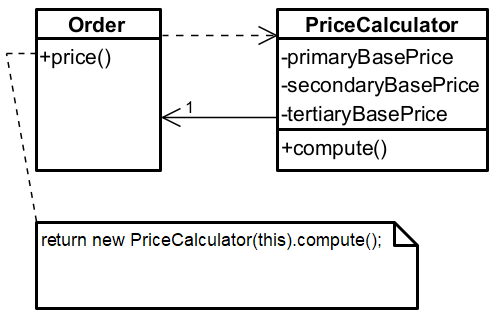
\includegraphics[width=0.45\textwidth]{methodToObject.png}
\end{center}

Уже неоднократно в этой лекции подчеркивалась прелесть небольших методов. Путем выделения в отдельные методы частей большого метода можно сделать код значительно более понятным. Но декомпозицию метода может затруднить наличие локальных переменных. Когда они присутствуют в изобилии, декомпозиция может оказаться сложной задачей. <<Замена временной переменной вызовом метода>> может облегчить ее, но иногда необходимое расщепление метода все же оказывается невозможным.

<<Замена метода объектом>> превращает локальные переменные в поля объекта методов. Затем к новому объекту применяется <<Выделение метода>>, создающее новые методы, на которые распадается первоначальный метод.

\subsection{Перемещение метода (Move Method)}

Метод чаще использует функции другого класса (или используется ими), а не того, в котором он определен. Создайте новый метод с аналогичным телом в том классе, который чаще всего им используется. Замените тело прежнего метода простым делегированием или удалите его вообще.

\begin{center}
    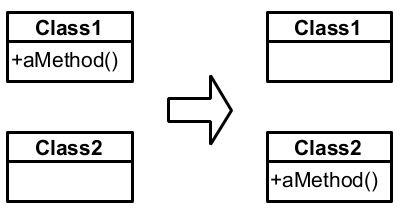
\includegraphics[width=0.4\textwidth]{moveMethod.png}
\end{center}

Перемещение методов~--- это насущный хлеб рефакторинга. Методы перемещают, если в классах сосредоточено слишком много функций или когда классы слишком плотно взаимодействуют друг с другом и слишком тесно связаны. Перемещая методы, можно сделать классы проще и добиться более четкой реализации функций. 

Обычно чтобы найти такие случаи, проглядывают методы класса, пытаясь обнаружить такой, который чаще обращается к другому объекту, чем к тому, в котором сам располагается. Особенно полезно это делать после перемещения каких-либо полей. Найдя подходящий для перемещения метод, рассмотрите, какие методы вызывают его, какими методами вызывается он сам, и поищите переопределяющие его методы в иерархии классов. 

Принять решение о перемещении не всегда просто. Если нет уверенности в необходимости перемещения данного метода, возможно имеет смысл перейти к рассмотрению других методов. Часто принять решение об их перемещении проще. Если принять решение трудно, то, вероятно, оно не столь уж и важно.

Если некоторая функция используется только тем методом, который вы собираетесь переместить, ее тоже вполне можно переместить. Если эта функция используется другими методами, посмотрите, нельзя ли и их переместить. Иногда проще переместить сразу группу методов, чем перемещать их по одному.

Проверьте, нет ли в подклассах и родительских классах исходного класса других объявлений метода. Если есть другие объявления, перемещение может оказаться невозможным, пока полиморфизм также не будет отражен в целевом классе.

\subsection{Выделение класса (Extract Class)}

Некоторый класс выполняет работу, которую следует поделить между двумя классами. Создайте новый класс и переместите соответствующие поля и методы из старого класса в новый.

\begin{center}
    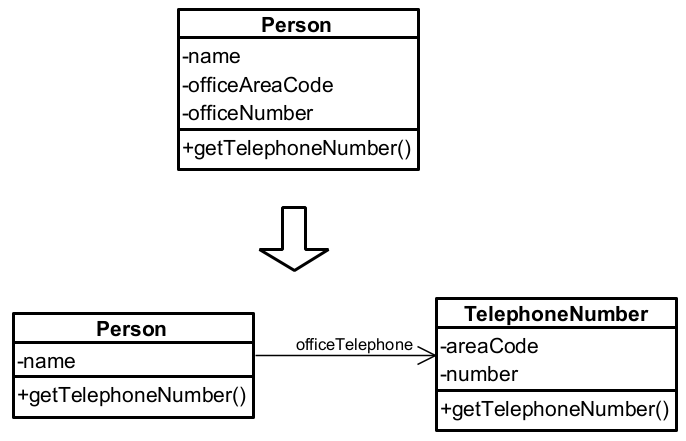
\includegraphics[width=0.7\textwidth]{extractClass.png}
\end{center}

Вероятно, вам приходилось слышать или читать, что класс должен представлять собой ясно очерченную абстракцию, выполнять несколько (в идеале одну) отчетливых обязанностей. На практике классы подвержены разрастанию. То добавится несколько операций, то появятся новые данные. Добавляя новые функции в класс, вы чувствуете, что для них не стоит заводить отдельный класс, но по мере того, как функции растут и плодятся, класс становится слишком сложным.

Получается класс с множеством методов и кучей данных, который слишком велик для понимания. Вы рассматриваете возможность разделить его на части и делите его. Хорошим признаком является сочетание подмножества данных с подмножеством методов. Другой хороший признак~--- наличие подмножеств данных, которые обычно совместно изменяются или находятся в особой зависимости друг от друга. Полезно задать себе вопрос о том, что произойдет, если удалить часть данных или метод. Какие другие данные или методы станут бессмысленны?

Одним из признаков, часто проявляющихся в дальнейшем во время разработки, служит характер создания подтипов класса. Может оказаться, что выделение подтипов оказывает воздействие лишь на некоторые функции или что для некоторых функций выделение подтипов производится иначе, чем для других.

Если обязанности прежнего класса перестают соответствовать его названию, переименуйте его. Может потребоваться двусторонняя ссылка, но не создавайте обратную ссылку, пока это не станет необходимо. Определите, должен ли новый класс быть выставлен наружу. Если да, то решите, как это должно быть сделано~--- в виде объекта ссылки или объекта с неизменяемым значением.

\subsection{Сокрытие делегирования (Hide Delegate)}

Клиент обращается к делегируемому классу объекта. Создайте на <<сервере>> методы, скрывающие делегирование.

\begin{center}
    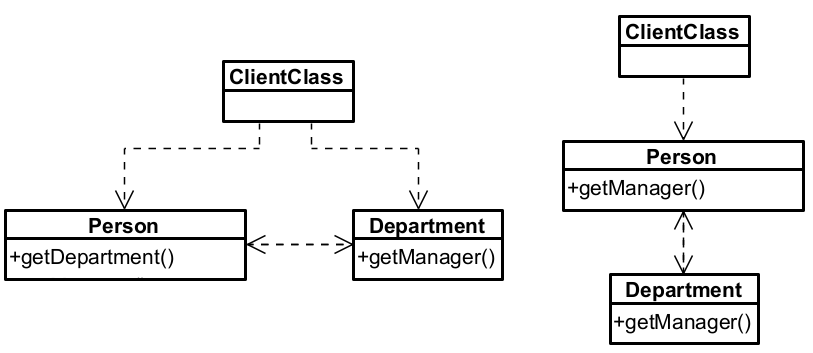
\includegraphics[width=0.8\textwidth]{hideDelegate.png}
\end{center}

Одним из ключевых свойств объектов является инкапсуляция. Инкапсуляция означает, что объектам приходится меньше знать о других частях системы. В результате при модификации других частей об этом требуется сообщить меньшему числу объектов, что упрощает внесение изменений.

Всякий, кто занимался ООП, знает, что поля следует скрывать, несмотря на то, что Java и другие языки позволяют делать поля открытыми. По мере роста искушенности в объектах появляется понимание того, что инкапсулировать можно более широкий круг вещей.

Если клиент вызывает метод, определенный над одним из полей объекта-сервера, ему должен быть известен соответствующий делегированный объект. Если изменяется делегированный объект, может потребоваться модификация клиента. От этой зависимости можно избавиться, поместив в сервер простой делегирующий метод, который скрывает делегирование. Тогда изменения ограничиваются сервером и не распространяются на клиента.

Может оказаться полезным применить <<Выделение класса>> к некоторым или всем клиентам сервера. Если скрыть делегирование от всех клиентов, можно убрать всякое упоминание о нем из интерфейса сервера.

\subsection{Введение внешнего метода (Introduce Foreign Method)}

Необходимо ввести в сервер дополнительный метод, но отсутствует возможность модификации класса. Создайте в классе клиента метод, которому в качестве первого аргумента передается класс сервера.

\begin{minted}{java}
Date newStart = new Date(previousEnd.getYear(),
    previousEnd.getMonth(), previousEnd.getDate() + 1);
\end{minted}

превращается в 

\begin{minted}{java}
Date newStart = nextDay(previousEnd);
static Date nextDay(Date arg) {
    return new Date (arg.getYear(), arg.getMonth(), arg.getDate() + 1);
}
\end{minted}

Ситуация достаточно распространенная. Есть прекрасный класс с отличными сервисами. Затем оказывается, что нужен еще один сервис, но класс его не предоставляет. А очень хочется. Если есть возможность модифицировать исходный код, вводится новый метод. Если такой возможности нет, приходится обходными путями программировать отсутствующий метод в клиенте.

Если клиентский класс использует этот метод единственный раз, то дополнительное кодирование не представляет больших проблем и, возможно, даже не требовалось для исходного класса. Однако если метод используется многократно, приходится повторять кодирование этого метода снова и снова. Повторение кода~--- корень всех зол в программах, поэтому повторяющийся код необходимо выделить в отдельный метод. При проведении этого рефакторинга можно явно известить о том, что этот метод в действительности должен находиться в исходном классе, сделав его внешним методом.

Не забывайте о том, что внешние методы являются искусственным приемом. По возможности старайтесь перемещать методы туда, где им надлежит находиться. Если проблема связана с правами владельца кода, отправьте внешний метод владельцу класса сервера и попросите его реализовать метод для вас.

Создаваемый метод не должен обращаться к каким-либо характеристикам клиентского класса. Если ему требуется какое-то значение, передайте его в качестве параметра.

\subsection{Самоинкапсуляция поля (Self Encapsulate Field)}

Обращение к полю осуществляется непосредственно, но взаимодействие с полем становится затруднительным. Создайте методы получения и установки значения поля и обращайтесь к полю только через них.

\begin{minted}{java}
private int _low, _high;

boolean includes(int arg) {
    return arg >= _low && arg <= _high;
}
\end{minted}

превращается в 

\begin{minted}{java}
private int _low, _high;

int getLow() { return _low; }
int getHigh() { return _high; }

boolean includes(int arg) {
    return arg >= getLow() && arg <= getHigh();
}
\end{minted}

Что касается обращения к полям, то здесь существуют две школы. Первая из них учит, что в том классе, где определена переменная, обращаться к ней следует свободно (непосредственный доступ к переменной). Другая школа утверждает, что даже внутри этого класса следует всегда применять методы доступа (косвенный доступ к переменной). Между двумя школами возникают горячие дискуссии.

В сущности, преимущество косвенного доступа к переменной состоит в том, что он позволяет переопределить в подклассе метод получения информации и обеспечивает большую гибкость в управлении данными, например отложенную инициализацию, при которой переменная инициализируется лишь при необходимости ее использования. Преимущество прямого доступа к переменной заключается в легкости чтения кода. Не надо останавливаться с мыслью: <<да это просто метод получения значения переменной>>.

Разумной рекомендацией тут будет действовать так, как считают нужным остальные участники команды. Действуя в одиночку, во избежание лишней работы имеет смысл сначала применять непосредственный доступ к переменной, пока это не становится препятствием. А при возникновении неудобств уже переходить на косвенный доступ к переменным. Рефакторинг предоставляет свободу изменить свое решение.

Важнейший повод применить <<Самоинкапсуляцию поля>> возникает, когда при доступе к полю родительского класса необходимо заменить обращение к переменной вычислением значения в подклассе. Первым шагом для этого является самоинкапсуляция поля. После этого можно заместить методы получения и установки значения теми, которые необходимы.

\subsection{Замена магического числа именованной константой}

Есть числовой, строковый или какой-то ещё литерал, имеющий определенный смысл. Создайте константу, дайте ей имя, соответствующее смыслу, и замените ею литерал.

\begin{minted}{java}
double potentialEnergy(double mass, double height) {
    return mass * 9.81 * height;
}
\end{minted}

превращается в 

\begin{minted}{java}
double potentialEnergy(double mass, double height) {
    return mass * GRAVITATIONAL_CONSTANT * height;
}

static final double GRAVITATIONAL_CONSTANT = 9.81;
\end{minted}

Магические числа~--- одна из старейших болезней в вычислительной науке. Это числа с особыми значениями, которые обычно не очевидны человеку со стороны. Магические числа очень неприятны, когда нужно сослаться на логически одно и то же число в нескольких местах. Если числа меняются, их модификация становится кошмаром. Даже если не требуется модификация, выяснить, что происходит, можно лишь с большим трудом.

Многие языки позволяют объявлять константы. При этом не наносится ущерб производительности и значительно улучшается читаемость кода.

Прежде чем выполнять этот рефакторинг, всегда стоит поискать возможную альтернативу. Посмотрите, как используется магическое число. Часто можно найти лучший способ его применения.

\subsection{Замена кода типа подклассами (Replace Type Code with Subclasses)}

Имеется неизменяемый код типа, воздействующий на поведение класса. Замените код типа подклассами.

\begin{center}
    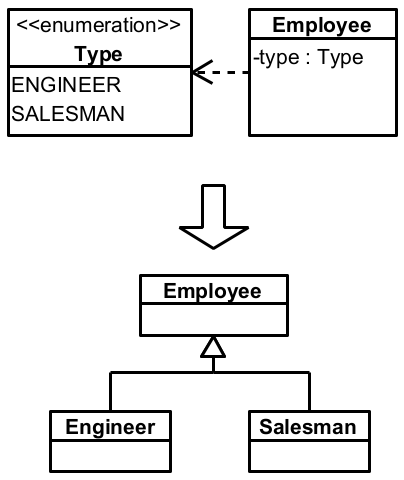
\includegraphics[width=0.4\textwidth]{replaceTypeCodeWithSubclass.png}
\end{center}

Если код типа не оказывает влияния на поведение, можно воспользоваться <<Заменой кода типа классом>>. Однако если код типа влияет на поведение, то вариантное поведение лучше всего организовать с помощью полиморфизма.

Обычно на такую ситуацию указывает присутствие условных операторов типа case. Это могут быть переключатели или конструкции типа if-then-else. В том и другом случае они проверяют значение кода типа и в зависимости от результата выполняют различные действия. К таким участкам кода должен быть применен рефакторинг <<Замена условного оператора полиморфизмом>>. Чтобы действовал данный рефакторинг, код типа должен быть заменен иерархией наследования, содержащей полиморфное поведение. В такой иерархии наследования имеются подклассы для каждого кода типа.

Простейший способ организовать такую структуру~--- <<Замена кода типа подклассами>>. Надо взять класс, имеющий этот код типа, и создать подкласс для каждого типа. Однако бывают случаи, когда сделать это нельзя. Один из них имеет место, когда код типа изменяется после создания объекта. Другой~--- при наличии класса, для кода типа которого уже созданы подклассы по другим причинам. В обоих случаях надо применять <<Замену кода типа состоянием/стратегией>>. <<Замена кода типа подклассами>> служит в основном вспомогательным шагом, позволяющим осуществить <<Замену условного оператора полиморфизмом>>. Побудить к применению <<Замены кода типа подклассами>> должно наличие условных операторов.

Другим основанием для <<Замены кода типа подклассами>> является наличие функций, относящихся только к объектам с определенными кодами типа. Осуществив этот рефакторинг, можно применить <<Спуск метода>> и <<Спуск поля>>, чтобы стало яснее, что эти функции касаются только определенных случаев.

<<Замена кода типа подклассами>> полезна тем, что перемещает осведомленность о вариантном поведении из клиентов класса в сам класс. При добавлении новых вариантов необходимо лишь добавить подкласс. В отсутствие полиморфизма пришлось бы искать все условные операторы и изменять их. Поэтому данный рефакторинг особенно полезен, когда варианты непрерывно изменяются.

\subsection{Замена кода типа Состоянием/Стратегией (Replace Type Code with State/Strategy)}

Этот рефакторинг сходен с <<Заменой кода типа подклассами>>, но может быть применен, когда код типа изменяется на протяжении существования объекта или если созданию подклассов мешают другие причины. В ней применяется паттерн <<Состояние>> или <<Стратегия>>.

Паттерны <<Состояние>> и <<Стратегия>> схожи в использовании, поэтому рефакторинг будет одинаковым в обоих случаях. Выберите тот паттерн, который лучше всего подходит в конкретной ситуации. Если вы пытаетесь упростить отдельный алгоритм с помощью <<Замены условного оператора полиморфизмом>>, лучше использовать <<Стратегию>>. Если вы собираетесь переместить специфические для состояния данные и представляете себе объект как изменяющий состояние, используйте паттерн <<Состояние>>.

\subsection{Замена условного оператора полиморфизмом (Replace Conditional with Polymorphism)}

Есть условный оператор, поведение которого зависит от типа объекта. Переместите каждую ветвь условного оператора в перегруженный метод подкласса. Сделайте исходный метод абстрактным.

\begin{minted}{java}
double getSpeed() {
    switch (_type) {
        case EUROPEAN:
            return getBaseSpeed();
        case AFRICAN:
            return getBaseSpeed() - getLoadFactor() * _numberOfCoconuts;
        case NORWEGIAN_BLUE:
            return _isNailed ? 0 : getBaseSpeed(_voltage);
    }
    throw new RuntimeException("Should be unreachable");
}
\end{minted}

превращается в

\begin{center}
    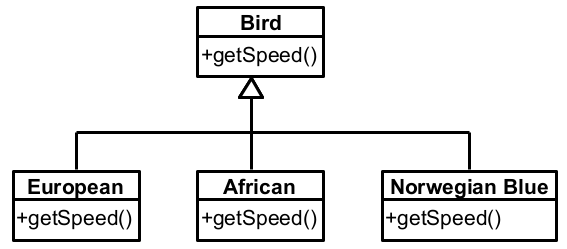
\includegraphics[width=0.5\textwidth]{replaceConditionalWithPolymorphism.png}
\end{center}

Одним из наиболее внушительно звучащих слов из жаргона объектного программирования является полиморфизм. Сущность полиморфизма состоит в том, что он позволяет избежать написания явных условных операторов, когда есть объекты, поведение которых различно в зависимости от их типа. В результате оказывается, что операторы switch, выполняющие переключение в зависимости от кода типа, или операторы if-then-else, выполняющие переключение в зависимости от строки типа, в объектно-ориентированных программах встречаются значительно реже.

Полиморфизм дает многие преимущества. Наибольшая отдача имеет место тогда, когда один и тот же набор условий появляется во многих местах программы. Если необходимо ввести новый тип, то приходится отыскивать и изменять все условные операторы. Но при использовании подклассов достаточно создать новый подкласс и обеспечить в нем соответствующие методы. Клиентам класса не надо знать о подклассах, благодаря чему сокращается количество зависимостей в системе и упрощается ее модификация.

\subsection{Введение Null-объекта (Introduce Null Object)}

Есть многократные проверки совпадения значения с null. Замените значение null Null-объектом.

\begin{minted}{java}
if (customer == null)
    plan = BillingPlan.basic();
else
    plan = customer.getPlan();
\end{minted}

превращается в

\begin{center}
    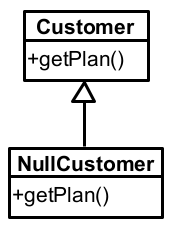
\includegraphics[width=0.15\textwidth]{nullObject.png}
\end{center}

Сущность полиморфизма в том, что вместо того, чтобы спрашивать у объекта его тип и вызывать то или иное поведение в зависимости от ответа, вы просто вызываете поведение. Объект, в зависимости от своего типа, делает то, что нужно. Всё это не так прозрачно, когда значением поля является null. 

Интересная особенность применения нулевых объектов состоит в том, что почти никогда не возникают аварийные ситуации. Поскольку нулевой объект отвечает на те же сообщения, что и реальный объект, система в целом ведет себя обычным образом. Из-за этого иногда трудно заметить или локализовать проблему, потому что все работает нормально. Конечно, начав изучение объектов, вы где-нибудь обнаружите нулевой объект, которого там быть не должно. 

\subsection{Разделение запроса и модификатора (Separate Query from Modifier)}

Есть метод, возвращающий значение, но, кроме того, изменяющий состояние объекта. Создайте два метода: один для запроса и один для модификации.

\begin{center}
    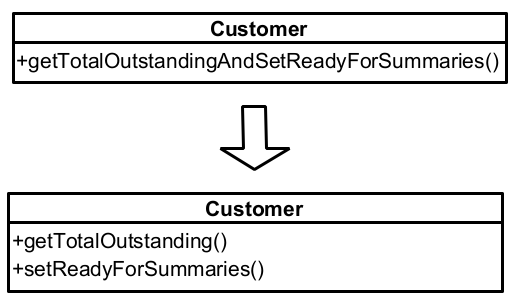
\includegraphics[width=0.5\textwidth]{separateQueryFromModifier.png}
\end{center}

Если есть функция, которая возвращает значение и не имеет видимых побочных эффектов, это весьма ценно. Такую функцию можно вызывать сколь угодно часто. Ее вызов можно переместить в методе в другое место. С ней значительно меньше проблем.

Хорошая идея~--- четко проводить различие между методами с побочными эффектами и теми, у которых их нет. Полезно следовать правилу, что у любого метода, возвращающего значение, не должно быть наблюдаемых побочных эффектов. Некоторые программисты рассматривают это правило как абсолютное. Можно и не придерживаться его в 100\% случаев (как и любых других правил), но в основном стараться его соблюдать весьма разумно.

Обнаружив метод, который возвращает значение, но также обладает побочными эффектами, следует попытаться разделить запрос и модификатор.

Возможно, вы обратили внимание на слова <<наблюдаемые побочные эффекты>>. Стандартная оптимизация заключается в кэшировании значения запроса в поле, чтобы повторные запросы выполнялись быстрее. Хотя при этом изменяется состояние объекта с кэшем, такое изменение не наблюдаемо. Любая последовательность запросов всегда возвращает одни и те же результаты для каждого запроса.

\subsection{Введение объекта-параметра (Introduce Parameter Object)}

Есть группа параметров, естественным образом связанных друг с другом. Замените их объектом.

\begin{center}
    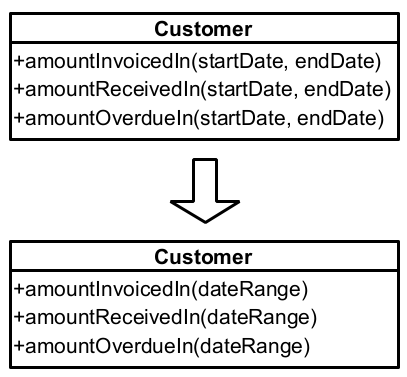
\includegraphics[width=0.4\textwidth]{introduceParameterObject.png}
\end{center}

Часто встречается некоторая группа параметров, обычно передаваемых вместе. Эта группа может использоваться несколькими методами одного или более классов. Такая группа классов представляет собой группу данных и может быть заменена объектом, хранящим все эти данные. Целесообразно свести эти параметры в объект, чтобы сгруппировать данные вместе. Такой рефакторинг полезен, поскольку сокращает размер списков параметров, а в длинных списках параметров трудно разобраться. Определяемые в новом объекте методы доступа делают также код более последовательным, благодаря чему его проще понимать и модифицировать.

Однако получаемая выгода ещё существеннее, поскольку после группировки параметров обнаруживается поведение, которое можно переместить в новый класс. Часто в телах методов производятся одинаковые действия со значениями параметров. Перемещая это поведение в новый объект, можно избавиться от значительного объема дублирующегося кода.

\subsection{Замена конструктора фабричным методом (Replace Constructor with Factory Method)}

Вы хотите при создании объекта делать нечто большее. Замените конструктор фабричным методом.

\begin{minted}{java}
Employee(int type) {
    _type = type;
}
\end{minted}

превращается в

\begin{minted}{java}
static Employee create(int type) {
    return new Employee(type);
}
\end{minted}

Самая очевидная мотивировка <<Замены конструктора фабричным методом>> связана с заменой кода типа созданием подклассов. Имеется объект, который обычно создается с кодом типа, но теперь требует подклассов. Конкретный подкласс определяется кодом типа. Однако конструкторы могут возвращать только экземпляр запрашиваемого объекта. Поэтому надо заменить конструктор фабричным методом. Фабричные методы можно использовать и в других ситуациях, когда возможностей конструкторов оказывается недостаточно. Их можно также применять для задания различных режимов создания, выходящих за рамки числа и типов параметров.

А ещё про это подробно пишет Блох в самой первой статье книги Effective Java.

\subsection{Подъем поля (Pull Up Field)}

В двух подклассах есть одинаковое поле. Переместите поле в родительский класс.

\begin{center}
    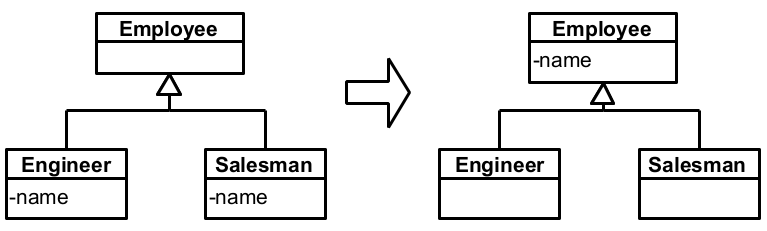
\includegraphics[width=0.8\textwidth]{pullUpField.png}
\end{center}

Если подклассы разрабатываются независимо или объединяются при проведении рефакторинга, в них часто оказываются дублирующиеся функции. В частности, дублироваться могут некоторые поля. Иногда у таких полей оказываются одинаковые имена, но это необязательно. Единственный способ разобраться в происходящем~--- посмотреть на поля и понять, как с ними работают другие методы. Если они используются сходным образом, можно их обобщить.

В результате дублирование уменьшается в двух отношениях. Удаляются дублирующиеся объявления данных и появляется возможность переместить из подклассов в родительский класс поведение, использующее поля.

Если поля закрытые, следует сделать поле родительского класса защищенным, чтобы подклассы могли ссылаться на него.

\subsection{Подъем метода (Pull Up Method)}

В подклассах есть методы с идентичными результатами. Переместите их в родительский класс.

\begin{center}
    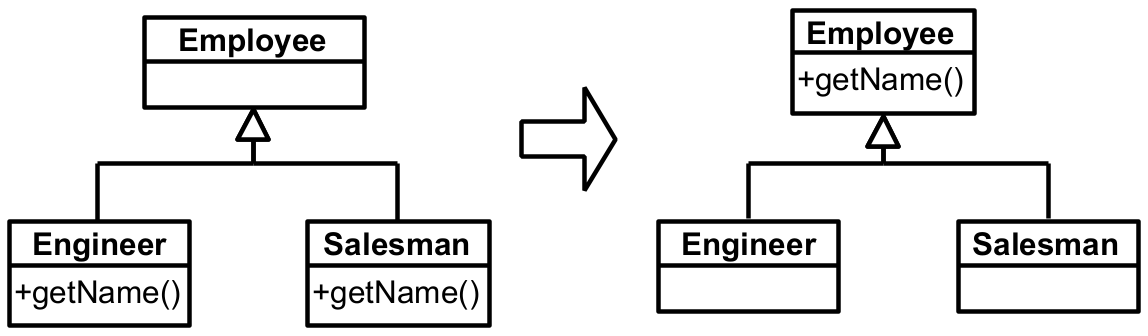
\includegraphics[width=0.8\textwidth]{pullUpMethod.png}
\end{center}

Дублирование поведения необходимо исключать. Хотя два дублирующихся метода прекрасно работают в существующем виде, они представляют собой питательную среду для возникновения ошибок в будущем. При наличии дублирования всегда есть риск, что при модификации одного метода второй будет пропущен. Обычно находить дубликаты трудно.

Простейший случай <<Подъема метода>> возникает, когда тела обоих методов одинаковы, что указывает на произведённые копирование и вставку. Конечно, ситуация не всегда столь очевидна. Можно просто выполнить рефакторинг и посмотреть, как пройдут тесты, но тогда придётся полностью положиться на свои тесты. Обычно бывает полезно поискать различия в методах, к которым применяется рефакторинг. Например, в них может обнаружиться поведение, протестировать которое забыли.

Часто условия для <<Подъема метода>> возникают после внесения некоторых изменений. Иногда в разных классах обнаруживаются два метода, которые можно параметризовать так, что они приводят, в сущности, к одному и тому же методу. Тогда, если двигаться самыми мелкими шагами, надо параметризовать каждый метод в отдельности, а затем обобщить их.

Особый случай <<Подъема метода>> возникает, когда некоторый метод подкласса перегружает метод родительского класса, но выполняет те же самые действия.

Самое неприятное в <<Подъеме метода>> то, что в теле методов могут быть ссылки на функции, находящиеся в подклассе, а не в родительском классе. Если функция представляет собой метод, можно обобщить и его, либо создать в родительском классе абстрактный метод. Чтобы это работало, может потребоваться изменить сигнатуру метода или создать делегирующий метод.

Если есть два сходных, но неодинаковых метода, можно попробовать выделить тут паттерн <<Шаблонный метод>>.

\subsection{Выделение подкласса (Extract Subclass)}

В классе есть функции, используемые только в некоторых случаях. Создайте подкласс для этого подмножества функций.

\begin{center}
    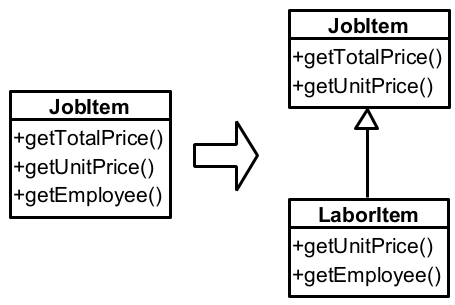
\includegraphics[width=0.4\textwidth]{extractSubclass.png}
\end{center}

Главным побудительным мотивом применения <<Выделения подкласса>> является осознание того, что в классе есть поведение, используемое в одних экземплярах и не используемое в других. Иногда об этом свидетельствует код типа, и тогда можно обратиться к <<Замене кода типа подклассами>> или <<Замене кода типа состоянием/стратегией>>. Но применение подклассов не обязательно предполагает наличие кода типа.

Основной альтернативой <<Выделению подкласса>> служит <<Выделение класса>>. Здесь нужно сделать выбор между делегированием и наследованием. <<Выделение подкласса>> обычно легче осуществить, но оно имеет некоторые ограничения. После того как объект создан, нельзя изменить его поведение, основанное на классе. Можно изменить основанное на классе поведение с помощью <<Выделения класса>>, просто подключая разные компоненты. Кроме того, для представления одного набора вариантов поведения можно использовать только подклассы. Если требуется, чтобы поведение класса изменялось несколькими разными способами, для всех из них, кроме одного, должно быть применено делегирование.

\subsection{Замена наследования делегированием (Replace Inheritance with Delegation)}

Подкласс использует только часть интерфейса родительского класса или не желает наследовать данные. Создайте поле для родительского класса, настройте методы, чтобы они делегировали выполнение родительскому классу, и удалите подклассы.

Наследование~--- замечательная вещь, но иногда это не совсем то, что нам требуется. Часто, осуществляя наследование класса, мы затем обнаруживаем, что многие из операций родительского класса в действительности неприемлемы для подкласса. В этом случае имеющийся интерфейс неправильно отражает то, что делает класс. Либо оказывается, что целая группа наследуемых данных неприемлема для подкласса. Либо обнаруживается, что в родительском классе есть защищенные методы, не имеющие особого смысла в подклассе.

Можно оставить все как есть и условиться говорить, что хотя это подкласс, но в нём используется лишь часть функций родительского класса. Но это приводит к коду, который говорит нечто, отличное от ваших намерений,~--- беспорядок, подлежащий неукоснительной ликвидации.

\begin{center}
    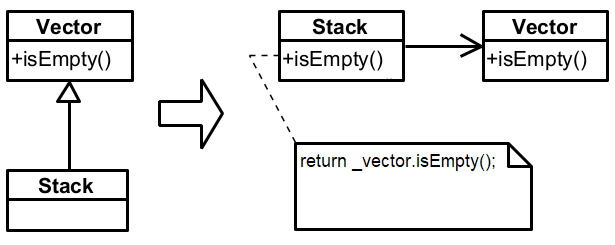
\includegraphics[width=0.7\textwidth]{replaceInheritanceWithDelegation.png}
\end{center}

Применяя вместо наследования делегирование, мы открыто заявляем, что используем делегируемый класс лишь частично. Мы управляем тем, какую часть интерфейса взять, а какую игнорировать. Цена этому~--- дополнительные делегирующие методы, писать которые скучно, но так просто, что трудно ошибиться.

\section{Когда нужно делать рефакторинг?}

Говоря о рефакторинге, имеет смысл затронуть вопрос о том, когда его проводить. Надо ли, например, выделять для проведения рефакторинга две недели после каждой пары месяцев работы?

Как правило, рефакторинг не стоит откладывать <<на потом>>. Рефакторингом следует заниматься постоянно понемногу. Надо не <<решать проводить рефакторинг>>, а проводить его, потому что необходимо сделать что-то еще, а поможет в этом рефакторинг.

\paragraph{Правило трех ударов.} Далее приводится полезный руководящий совет из книги Мартина Фаулера. Делая что-то в первый раз, вы просто это делаете. Делая что-то аналогичное во второй раз, вы морщитесь от необходимости повторения, но все-таки повторяете то же самое. Делая что-то похожее в третий раз, вы начинаете рефакторинг.

\paragraph{Применяйте рефакторинг при добавлении новой функции.} Чаще всего рефакторинг производится, когда в некоторое программное обеспечение требуется добавить новую функцию. Иногда при этом причиной рефакторинга является желание лучше понять код, который надо модифицировать. Этот код мог написать кто-то другой, а может и вы сами. Всякий раз, когда приходится думать о том, что делает некий код, задайте себе вопрос о том, можете ли вы изменить его структуру так, чтобы организация кода стала более очевидной. После этого проведите рефакторинг кода. Отчасти это делается на тот случай, если вам снова придется с ним работать, но в основном потому, что вам большее становится понятным, если в процессе работы код делается более ясным.

Еще одна причина, которая в этом случае побуждает к проведению рефакторинга,~--- это дизайн, не способствующий легкому добавлению новой функции. Вы смотрите на архитектуру кода и понимаете, что если бы он был спроектирован так-то и так-то, добавить такую функцию было бы проще. В таком случае не надо переживать о прежних промахах, а просто исправлять их путём проведения рефакторинга. После правильного рефакторинга добавление новой функции происходит значительно более гладко и занимает меньше времени.

\paragraph{Применяйте рефакторинг, если требуется исправить ошибку.} При исправлении ошибок польза рефакторинга во многом заключается в том, что код становится более понятным. Мы смотрим на код, пытаясь понять его, и мы производим рефакторинг кода, чтобы лучше понять. Часто оказывается, что такая активная работа с кодом помогает найти в нем ошибки. Можно взглянуть на это и так: если мы получаем сообщение об ошибке, то это признак необходимости рефакторинга, потому что код не был достаточно ясным и мы не смогли увидеть ошибку.

\paragraph{Применяйте рефакторинг при ревью кода.} Благодаря ревью кода знания о системе становятся достоянием всей команды разработчиков. При этом более опытные разработчики передают свои знания менее опытным. Ревью помогают большему числу людей разобраться с большим числом аспектов крупной программной системы. Они также очень важны для написания понятного кода. Мой код может казаться понятным мне, но не моей команде. Это неизбежно: очень трудно поставить себя на место того, кто не знаком с вашей работой. Ревью также дают возможность большему числу людей высказать полезные мысли.

Рефакторинг помогает вам разобраться в коде, написанном не вами. Когда в процессе ревью у вас возникают идеи, можно сразу смотреть, нельзя ли их тут же реализовать с помощью рефакторинга. Если да, то можно сразу и провести его. Проделав это несколько раз, вы будете лучше понимать, как будет выглядеть код после внесения в него предлагаемых изменений. Не надо напрягать воображение, чтобы увидеть будущий код, это можно сделать уже теперь. В результате появляются уже идеи следующего уровня, которых у вас не возникло бы, не проведи вы рефакторинг.

Кроме того, рефакторинг способствует получению более конкретных результатов от разбора кода. В его процессе не только возникают новые предложения, но многие из них тут же реализуются. В результате это мероприятие дает ощущение большей успешности.

\section{Проблемы, возникающие при проведении рефакторинга}

При изучении новой технологии, повышающей производительность труда, бывает нелегко увидеть, что есть случаи, когда она неприменима. Обычно она изучается в особом контексте, часто являющемся отдельным проектом. Трудно увидеть, почему технология может стать менее эффективной и даже вредной. Нам известно, какие выгоды приносит рефакторинг. Нам известно, что они могут ощутимо изменить нашу работу. Но наш опыт еще недостаточно богат, чтобы увидеть, какие ограничения присущи рефакторингу.

\subsection{Работа с данными}

Одной из областей применения рефакторинга служат базы данных. Большинство деловых приложений тесно связано с поддерживающей их схемой базы данных. Это одна из причин, по которым базу данных трудно модифицировать. Другой причиной является миграция данных. Даже если система тщательно разбита по слоям, чтобы уменьшить зависимости между схемой базы данных и объектной моделью, изменение схемы базы данных вынуждает к миграции данных, что может оказаться длительной и рискованной операцией.

В случае необъектных баз данных с этой задачей можно справиться, поместив отдельный программный слой между объектной моделью и моделью базы данных. Благодаря этому можно отделить модификации двух разных моделей друг от друга. Внося изменения в одну модель, не обязательно изменять другую, надо лишь модифицировать промежуточный слой. Такой слой вносит дополнительную сложность, но дает значительную гибкость. Даже без проведения рефакторинга это очень важно в ситуациях, когда имеется несколько баз данных или сложная модель базы данных, управлять которой вы не имеете возможности.

Объектные модели одновременно облегчают задачу и усложняют ее. Некоторые объектно-ориентированные базы данных позволяют автоматически переходить от одной версии объекта к другой. Это сокращает необходимые усилия, но влечет потерю времени, связанную с осуществлением перехода. Если переход не автоматизирован, его приходится осуществлять самостоятельно, что требует больших затрат. В этом случае следует более осмотрительно изменять структуры данных классов. Можно свободно перемещать методы, но необходимо проявлять осторожность при перемещении полей. Надо применять методы для доступа к данным, чтобы создавать иллюзию их перемещения, в то время как в действительности его не происходило. При достаточной уверенности в том, где должны находиться данные, можно переместить их с помощью одной операции. Модифицироваться должны только методы доступа, что снижает риск появления ошибок.

\subsection{Изменение интерфейсов}

Важной особенностью объектов является то, что они позволяют изменять реализацию программного модуля независимо от изменений в интерфейсе. Можно благополучно изменить внутреннее устройство объекта, никого при этом не потревожив, но интерфейс имеет особую важность: если изменить его, может случиться всякое. В рефакторинге беспокойство вызывает то, что во многих случаях интерфейс действительно изменяется. Такие простые вещи, как <<Переименование метода>>, целиком относятся к изменению интерфейса. Как это соотносится с бережно хранимой идеей инкапсуляции?

Поменять имя метода нетрудно, если доступен весь код, вызывающий этот метод. Даже если метод открытый, но можно добраться до всех мест, откуда он вызывается, и модифицировать их, метод можно переименовывать. Проблема возникает только тогда, когда интерфейс опубликован, то есть используется кодом, который не доступен для изменений. Если интерфейс опубликован, изменять его и просто редактировать точки вызова небезопасно. Необходима несколько более сложная технология. При таком взгляде вопрос изменяется. Теперь задача формулируется следующим образом: как быть с рефакторингами, изменяющими опубликованные интерфейсы? 

При изменении опубликованного интерфейса в процессе рефакторинга необходимо сохранять как старый интерфейс, так и новый, по крайней мере до тех пор, пока пользователи не смогут отреагировать на модификацию. К счастью, это не очень трудно. Обычно можно сделать так, чтобы старый интерфейс продолжал действовать. Попытайтесь устроить так, чтобы старый интерфейс вызывал новый. При этом, изменив название метода, сохраните прежний. Не копируйте тело метода. При разработке на Java, например, следует также воспользоваться средством пометки кода как устаревшего (необходимо объявить метод, который более не следует использовать, с модификатором deprecated). Благодаря этому обращающиеся к коду будут знать, что ситуация изменилась.

Защита интерфейсов обычно осуществима, но связана с усилиями. Необходимо создать и сопровождать эти дополнительные методы, по крайней мере, временно. Эти методы усложняют интерфейс, затрудняя его применение. Однако есть альтернатива: не публикуйте интерфейс. Никто не говорит здесь о полном запрете; ясно, что опубликованные интерфейсы должны быть. Если вы создаете API для внешнего использования, как это делает Oracle, то тогда у вас должны быть опубликованные интерфейсы.

Есть ещё одна особая область проблем, возникающих в связи с изменением интерфейсов в Java: добавление исключительной ситуации в предложения throw объявлений методов. Это не изменение сигнатуры, поэтому ситуация не решается с помощью делегирования. Однако компилятор не позволит осуществить компиляцию. С данной проблемой бороться тяжело. Можно создать новый метод с новым именем, позволить вызывать его старому методу и превратить обрабатываемую исключительную ситуацию в необрабатываемую. Можно также генерировать необрабатываемую исключительную ситуацию, хотя при этом теряется возможность проверки. Если так поступить, можно предупредить тех, кто пользуется методом, что исключительная ситуация в будущем станет обрабатываемой, дав им возможность установить обработчики в своем коде. Одни из решений может быть определение родительского класса исключительных ситуаций для пакета в целом (например, SQLException для java.sql) и объявление этой исключительной ситуации только в предложениях throw опубликованных методов. Используя такой подход, возможно создать иерархию классов исключительных ситуаций и использовать только родительский класс в предложениях throw опубликованных интерфейсов, в то же время можно будет использовать его подклассы в более специфичных ситуациях посредством операций приведения и проверки типа объекта исключительной ситуации. Благодаря этому при желании можно определять подклассы исключительных ситуаций, что не затрагивает вызывающего, которому известен только общий случай.

\subsection{Глобальные изменения архитектуры}

Можно ли с помощью рефакторинга исправить любые недостатки проектирования или в дизайне системы могут быть заложены такие базовые решения, которые впоследствии не удастся изменить путем проведения рефакторинга? Имеющиеся в этой области данные недостаточны. Конечно, часто рефакторинг оказывается эффективным, но иногда возникают трудности.

Осторожно-разумный подход состоит в том, чтобы представить себе возможный рефакторинг. Рассматривая различные варианты дизайна системы, попытайтесь определить, насколько трудным окажется рефакторинг одного дизайна в другой. Если трудностей не видно, то можно, не слишком задумываясь о выборе, остановиться на самом простом дизайне, даже если он не охватывает все требования, которые могут возникнуть в дальнейшем. Однако если простых способов рефакторинга найти не удаётся, то надо дальше работать над дизайном.

\subsection{Рефакторинг и производительность}

С рефакторингом обычно связан вопрос о его влиянии на производительность программы. С целью облегчить понимание работы программы часто осуществляется модификация, приводящая к замедлению выполнения программы. Это важный момент. Рефакторинг, несомненно, иногда заставляет программу выполняться несколько медленнее, но при этом делает ее более податливой для настройки производительности. Секрет создания быстрых программ, если только они не предназначены для работы в жестком режиме реального времени, состоит в том, чтобы сначала написать программу, которую можно настраивать, а затем настроить ее так, чтобы достичь приемлемой скорости.

Известны три подхода к написанию быстрых программ. Наиболее трудный из них связан с ресурсами времени и часто применяется в системах с жесткими требованиями к выполнению в режиме реального времени. В этой ситуации при декомпозиции проекта каждому компоненту выделяется бюджет ресурсов~--- по времени и памяти. Компонент не должен выйти за рамки своего бюджета, хотя разрешен механизм обмена временными ресурсами. Такой механизм жестко сосредоточен на соблюдении времени выполнения. Это важно в таких системах, как, например, кардиостимуляторы, в которых данные, полученные с опозданием, всегда ошибочны. Данная технология избыточна в системах другого типа, например в корпоративных информационных системах, которых создаётся великое множество.

Второй подход предполагает постоянное внимание. В этом случае каждый программист в любой момент времени делает всё от него зависящее, чтобы поддерживать высокую производительность программы. Это распространенный и интуитивно привлекательный подход, однако он не так хорош на деле. Модификация, повышающая производительность, обычно затрудняет работу с программой. Это замедляет создание программы. На это можно было бы пойти, если бы в результате получалось более быстрое программное обеспечение, но обычно этого не происходит. Повышающие скорость усовершенствования разбросаны по всей программе, и каждое из них касается только узкой функции, выполняемой программой.

С производительностью связано то интересное обстоятельство, что при анализе большинства программ обнаруживается, что большая часть времени расходуется небольшой частью кода. Если в равной мере оптимизировать весь код, то окажется, что 90\% оптимизации произведено впустую, потому что оптимизировался код, который выполняется не слишком часто. Время, ушедшее на ускорение программы, и время, потерянное из-за ее непонятности~--- всё это израсходовано напрасно.

Третий подход к повышению производительности программы основан как раз на этой статистике. Он предполагает создание программы с достаточным разложением её на компоненты без оглядки на достигаемую производительность вплоть до этапа оптимизации производительности, который обычно наступает на довольно поздней стадии разработки и на котором осуществляется особая процедура настройки программы.

Начинается всё с запуска программы под профайлером, контролирующим программу и сообщающим, где расходуются время и память. Благодаря этому можно обнаружить тот небольшой участок программы, в котором находятся узкие места производительности. На этих узких местах сосредоточиваются усилия, и осуществляется та же самая оптимизация, которая была бы применена при подходе с постоянным вниманием. Но благодаря тому, что внимание сосредоточено на выявленных узких местах, удается достичь больших результатов при значительно меньших затратах труда. Но даже в этой ситуации необходима бдительность. Как и при проведении рефакторинга, изменения следует вносить небольшими порциями, каждый раз компилируя, тестируя и запуская профайлер. Если производительность не увеличилась, изменения надо откатить. Процесс поиска и ликвидации узких мест продолжается до достижения производительности, которая удовлетворяет пользователей.

Хорошее разделение программы на компоненты способствует оптимизации такого рода в двух отношениях. Во-первых, благодаря ему появляется время, которое можно потратить на оптимизацию. Имея хорошо структурированный код, можно быстрее добавлять новые функции и выиграть время для того, чтобы заняться производительностью. Профилирование гарантирует, что это время не будет потрачено зря. Во-вторых, хорошо структурированная программа обеспечивает более высокое разрешение для анализа производительности. Профайлер указывает на более мелкие фрагменты кода, которые легче настроить. Благодаря большей понятности кода легче осуществить выбор возможных вариантов и разобраться в том, какого рода настройка может оказаться действенной.

\section{Когда рефакторинг не нужен?}

В некоторых случаях рефакторинг вообще не нужен. Основной пример~--- необходимость переписать программу с нуля. Иногда имеющийся код настолько запутан, что подвергнуть его рефакторингу, конечно, можно, но проще начать всё с самого начала. Но такое решение принять нелегко, и тут мы его не будем рассматривать.

Явный признак необходимости переписать код~--- его неработоспособность. Это обнаруживается только при его тестировании, когда ошибок оказывается так много, что сделать код устойчивым не удается. Помните, что перед началом рефакторинга код должен выполняться в основном корректно.

Компромиссное решение состоит в создании компонентов с сильной инкапсуляцией путем рефакторинга значительной части программного обеспечения. После этого для каждого компонента в отдельности можно принять решение относительно изменения его структуры при помощи рефакторинга или воссоздания заново. Это особенно привлекательный подход, когда основная система является унаследованной.

Другой случай, когда следует воздерживаться от рефакторинга, это близость даты завершения проекта. Рост производительности, достигаемый благодаря рефакторингу, проявит себя слишком поздно, после истечения срока. Уорд Каннингем незавершенный рефакторинг сравнивает с залезанием в долги. Большинству компаний для нормальной работы нужны кредиты. Однако вместе с долгами появляются и проценты, то есть дополнительная стоимость обслуживания и расширения, обусловленная чрезмерной сложностью кода. Выплату каких-то процентов можно вытерпеть, но если платежи слишком велики, вы разоритесь. Важно управлять своими долгами, выплачивая их часть посредством рефакторинга.

\end{document}